\documentclass[pdflatex,sn-apa]{sn-jnl}

\usepackage{graphicx}
\usepackage{amsmath,amssymb}
\usepackage{booktabs}
\usepackage{multirow}
\usepackage{xcolor}
\usepackage{textcomp}

\raggedbottom

\begin{document}

\title[Unconcentrated markets, captive buyers]{Unconcentrated markets, captive buyers: incumbency in Türkiye's public IT procurement}

\author*[1]{\fnm{Furkan} \sur{Aksoy}}\email{furkan78177@gmail.com}
\author[1]{\fnm{Arda} \sur{Şimşek}}\email{simsekarda5803@gmail.com}

\affil*[1]{\orgdiv{Department of Software Engineering}, \orgname{Maltepe University}, \orgaddress{\city{Istanbul}, \country{Türkiye}}}

\abstract{Market-level concentration indices are the standard screen for competition problems in public procurement, yet a market can be unconcentrated while many of its buyers depend on a single supplier. We examine this gap using 9,991 awarded information-technology (IT) contracts published on Türkiye's electronic procurement platform EKAP between 2010 and 2026, linking 2,814 firms to 2,890 public buyers. After auditing the IT scope by contract value, resolving firm-name variants, and deflating values, no product market is robustly concentrated: supplier Herfindahl--Hirschman indices stay below 1,000 once count, real value, and the influence of single contracts are taken into account, with health information systems the closest case. Buyers, however, return to their previous suppliers far more often than chance predicts. Among contracts awarded by a buyer that has bought in the same product market before, 45\% go to an incumbent supplier, compared with 6\% under a permutation null that preserves each buyer's demand and each firm's wins within product market and year; the excess remains 2.2-fold under a null that also fixes the province. More than half of buyers with at least five contracts are more dependent on their main supplier than their own null distribution allows. Incumbency is strongest in health IT and in negotiated procurement without prior publication (Article 21(b) of Law 4734), where it rose markedly after 2017, and incumbent-won tenders are far more likely to attract a single bid. We argue that buyer-level incumbency measures belong alongside market concentration in procurement monitoring.}

\keywords{Public procurement, Incumbency, Vendor lock-in, Market concentration, Bipartite networks, Türkiye}

\pacs[JEL Classification]{H57, L14, L86, D85}

\maketitle

\section{Introduction}\label{sec:intro}

Competition authorities and procurement regulators usually begin with market structure. The Herfindahl--Hirschman index (HHI) and concentration ratios summarize how supply is shared among firms in a relevant market, and fixed thresholds translate them into a first judgement about competitive risk \citep{hirschman1964,rhoades1993,MergerGuidelines2023}. In public procurement this screen has a specific blind spot. A market can contain many suppliers, none with a large share, while individual public buyers keep returning to the same firm. Market-level shares are then low, but the relevant choice for each buyer is narrow. Switching costs, installed systems, and procedural discretion can sustain such buyer-level dependence without producing market-level concentration \citep{klemperer1995,FarrellKlemperer2007,Greenstein1993}.

This paper documents that gap for the public IT market of Türkiye. IT procurement is a natural setting because installed software and hardware create switching costs, because public services increasingly depend on a small number of information systems, and because Turkish law provides a negotiated route without prior publication (Article 21(b) of Public Procurement Law No.~4734) that can be used where only one supplier is deemed able to deliver. We reconstruct 9,991 awarded IT contracts from the national e-procurement platform EKAP (2010--2026) as a network of 2,814 firms and 2,890 buyers, and ask three questions. Is the market concentrated once it is measured carefully? Do buyers return to incumbent suppliers more often than market structure alone would produce? And where, and under which procedures, is such incumbency strongest?

The answers are as follows. First, no product market is robustly concentrated. Pooled supplier HHI is 39 by contract count and 149 by real value, and within product markets the count-based index stays below 1,000 everywhere. Value-based indices exceed 1,000 only where a single very large contract dominates a small market, and they fall below the threshold once that contract is removed. Health information systems, the largest market, is the closest to moderate concentration. Second, incumbency is pervasive. Among contracts awarded by a buyer that has bought in the same product market before, 45.2\% go to a firm that already supplied that buyer in that market. A permutation null that keeps each buyer's demand and each firm's wins within product market and year predicts 6.2\%. The excess survives nulls that also condition on buyer sector (4.1-fold) and province (2.2-fold), and 57\% of buyers with at least five contracts exceed their own null in dependence on their main supplier. Third, incumbency is strongest in health IT, particularly among individual Ministry of Health hospitals, and in Article~21(b) procurement. There, the incumbency rate rose from 54\% before 2018 to 81\% afterwards, although the timing of this rise cannot be attributed to a single legal change. In a year-stratified sample of tenders with published bid counts, incumbent-won tenders attracted a single bid 71\% of the time, against 32\% for tenders won by new suppliers.

The paper contributes in three ways. Recent work has begun to combine concentration measures with network analysis of procurement markets, showing that entropy- or HHI-based indices and centrality can point in different directions \citep{Fountoukidis2023,Pliatsidis2024,Fountoukidis2026}. We build on this work by testing the buyer--supplier layer against explicit null models rather than describing it, which separates relational persistence from the mechanical dilution of pooled indices across heterogeneous markets. Second, we provide the first network-based evidence on Turkish public IT procurement. We add to a literature that has so far focused on political connections and construction \citep{Gurakar2016,GurakarBircan2019,KutlayYildirim2024}. Third, we offer a reproducible pipeline for EKAP data, including a value-based audit of keyword-defined scope that removes a substantial share of non-IT spending that keyword searches admit.

\section{Background and related literature}\label{sec:background}

\subsection{Concentration, switching costs, and incumbency}
The HHI is informative only relative to a relevant market; pooled across markets that are not substitutes, it is mechanically diluted because each firm's share is divided among unrelated demand \citep{rhoades1993}. In procurement, the relevant choice set may be even narrower than a product market. A hospital that has installed a hospital information system faces data-migration, training, and integration costs if it changes supplier, and these costs create the lock-in described in the switching-cost literature \citep{klemperer1995,FarrellKlemperer2007,ShapiroVarian1999}. \citet{Greenstein1993} shows for US federal computer procurement that installed base strongly predicts the choice of vendor. Incumbency advantages in public contracting have also been documented where buyers have discretion \citep{Coviello2018,CovielloGagliarducci2017} and in the dynamics of repeated procurement auctions \citep{KangMiller2022}. Negotiation rather than competitive bidding can be efficient for complex, customized purchases \citep{Bajari2009}, so repeated contracting is not by itself evidence of harm. Discretion can improve performance when it lets buyers rely on proven suppliers \citep{Coviello2018}. The empirical question is therefore how much incumbency exists beyond what market structure implies, and where.

\subsection{Procurement as a network}
Contract-award records are naturally two-mode: buyers award contracts to suppliers. Network studies of procurement have used this structure to study corruption risk and favoritism \citep{wachs2019corr,FazekasWachs2020}, to detect collusion from co-bidding networks \citep{wachs2019cartel,ReevesLatourMorselli2017}, and to characterize the structure of buyer--supplier transactions \citep{Popa2019}. The integrity literature builds objective risk indicators from award data, most prominently the single-bidding rate \citep{fazekas2016objective,FazekasKocsis2020}. Closest to our question, \citet{Fountoukidis2023} show for the European pacemaker market that concentration-type indices can indicate competition while network centrality reveals dominant suppliers, and \citet{Pliatsidis2024} measures concentration in Greek procurement with network methods by product group. We share their premise that market shares and network structure can diverge. We differ in the object and the test. Our object is the buyer--supplier tie rather than node centrality, and we test its persistence against permutation nulls that hold market structure fixed.

\subsection{The Turkish context}
Turkish public procurement is governed by Law No.~4734 (2002) and administered by the Public Procurement Authority (KİK), whose electronic platform EKAP publishes notices and award results \citep{alsac2017}. Article~21 of the law lists negotiated procedures. Article~21(b) permits negotiation without prior publication where urgent needs or exclusive capabilities make a competitive procedure impractical. Its use has been debated in Turkish legal scholarship \citep{Alyanak2022}, and Law No.~7144 (in force 25 May 2018) extended the cases in which buyers may invoke it. Political economy studies document that politically connected firms win more often under less competitive procedures \citep{Gurakar2016,GurakarBircan2019} and that market capture intensified during the 2010s \citep{KutlayYildirim2024}; see also \citet{BugraSavaskan2014}. These studies focus mainly on construction and on political connections; the IT market and the buyer-level structure of repeat contracting have not been examined. The health sector also underwent a major reorganization during our window. Decree-Law (KHK) No.~694 abolished the Public Hospitals Authority and its provincial hospital unions on 25 August 2017, returning hospital procurement to the Ministry of Health and to individual hospitals.

\section{Data}\label{sec:data}

\subsection{Collection and scope}
We collected award records of IT-related tenders from EKAP using domain keywords and retained those concluded with an identifiable winner (13,418 records before cleaning). Keyword search on EKAP matches substrings, so it admits tenders whose titles contain an IT term only incidentally. The term \emph{ERP}, for example, matches place names and \emph{tuz serpici} (salt spreader), and \emph{technical support} matches hospital staffing contracts. A count-based audit had suggested that such false positives were rare; a value-based audit showed they were not. We therefore reviewed the 150 largest contracts by value manually, derived title-based rules for the remainder, and spot-checked random samples by rule. Of the 13,024 contracts that had passed an earlier count-based cleaning step, 1,627 (12.5\%, holding 17.7\% of nominal value) are not IT: housing construction, mining overburden removal, vehicles, and cleaning staff, among others. A further 1,406 are ambiguous (for example hospital data-entry staffing or building works that include security cameras). Our main sample contains the 9,981 unambiguous IT contracts plus 10 contracts for IT-enabled call-centre services, one of which, the national hospital appointment system (MHRS) call-centre contract of 2025, is by far the largest in the data. All results are reported with and without this contract. The ambiguous group is used as a robustness sample.

\subsection{Entities, markets, and values}
Firms appear on EKAP under spelling and legal-form variants. We canonicalized names by normalizing characters and removing legal-form suffixes, and we reviewed the merge groups of the 300 largest firms by hand, keeping joint ventures separate. This reduces 4,788 recorded names to 4,389 firms overall and to 2,814 firms in the main sample. Some public buyers are recorded under generic labels that pool units across provinces, most notably the provincial health directorates of the Ministry of Health. We split such labels by the province recorded for each tender (36 labels, 1,001 contracts) and use the recorded labels as a sensitivity check. This yields 2,890 buyers in the main sample. We assign each contract to one of 14 product markets from its title (for example health information systems, enterprise software, network infrastructure, software licences, and GIS) and each buyer to one of 11 buyer sectors. Values are deflated to 2025 lira with the annual consumer price index. About 536 winners are natural persons (sole proprietors); in the released data they are pseudonymized. Table~\ref{tab:data} summarizes the main sample.

\begin{table}[t]
\caption{Main sample (IT and IT-enabled services, EKAP 2010--2026).}\label{tab:data}
\begin{tabular}{@{}lr@{}}
\toprule
Awarded contracts & 9,991\\
Firms (canonicalized) & 2,814\\
Buyers (pooled labels split by province) & 2,890\\
Buyer--firm pairs (dyads) & 7,219\\
Dyads with two or more contracts & 1,377 (19.1\%)\\
Contracts in repeat dyads & 41.5\%\\
Total value, 2025 TRY (nominal TRY) & 89.3 bn (33.3 bn)\\
Largest contract (MHRS call centre, 2025), share of real value & 8.4\%\\
Contracts under Article 21(b) & 1,048 (10.5\%)\\
Tender dates & Oct 2010 -- Mar 2026\\
\botrule
\end{tabular}
\end{table}

\section{Methods}\label{sec:methods}

\subsection{Concentration}
For each product market we compute the supplier HHI, $H=\sum_i s_i^2$ on a 0--10,000 scale, and the four-firm ratio CR4, using contract counts and real values. Because single contracts can dominate value shares, we also report value-based HHI without the market's largest contract, the maximum change from removing any single contract, and a variant with contract values winsorized at the 99th percentile. Confidence intervals come from 1,000 bootstrap resamples of contracts within market; because the plug-in HHI is biased upward under resampling, we report bias-shifted percentile intervals. We also compute HHI within calendar years, where values need no deflation. We classify markets against the 2023 US Merger Guidelines thresholds of 1,000 and 1,800 \citep{MergerGuidelines2023}, noting that these are screening thresholds for mergers, not measures of conduct. Finally, we decompose the pooled index as $H_{\text{agg}} = \sum_m w_m^2 H_m + C$, where $w_m$ is the share of market $m$ and $C$ collects the cross-market terms of firms active in several markets. The decomposition makes explicit how much of the gap between pooled and market-level concentration is mechanical.

\subsection{Incumbency and null models}
Let contract $i$ be awarded by buyer $k$ in product market $m$ on date $t$. Contract $i$ is \emph{repeat-eligible} if $k$ awarded at least one other contract in $m$ strictly before $t$, and it is \emph{incumbent} if its winner had already won a contract from $k$ in $m$ strictly before $t$. The incumbency rate is the share of repeat-eligible contracts that are incumbent. Eligibility depends only on buyer, market, and date, so the eligible set is fixed across permutations.

To separate incumbency from market structure, we permute winner labels across contracts within cells and recompute all statistics. Under null N1 the cells are product market $\times$ calendar year. Each buyer's demand in each cell and each firm's number of wins in each cell are preserved, so firm entry and exit, market specialization, and market size are held fixed; only the assignment of winners to buyers is randomized. Null N2 adds the buyer sector to the cell and N3 adds the province, which absorbs local supplier pools. Each null uses 1,000 permutations with fixed seeds. We report the observed value, the null mean and 95\% interval, the ratio of observed to null, and a one-sided permutation $p$-value, whose minimum with 1,000 draws is 0.001. Subgroups (market, sector, procedure, period) are compared with the same permutation draws restricted to the subgroup, so each subgroup has its own baseline. For buyer-level dependence we compute, for the 540 buyers with at least five contracts, the share of the main supplier and the supplier HHI of the buyer's purchases, and compare each buyer with its own null distribution.

\subsection{Correlates of incumbency}
We model the probability that a repeat-eligible contract is won by an incumbent with a logit that includes the procedure (Article~21(b), other negotiated procedures, open as reference), a post-2018 indicator and its interaction with 21(b), the log real value, the buyer's number of prior contracts and prior distinct suppliers in the market, the years since the buyer's first contract in the market, and product-market, year, and buyer-sector fixed effects. Standard errors are clustered two ways, by buyer and by winning firm \citep{Cameron2011}. We report average marginal effects, a linear probability model with buyer fixed effects, and alternative break dates. A secondary model follows each new buyer--firm pair from its first contract and asks whether it continues; it is described in the Supplementary Information together with its specification tests.

\subsection{Single bidding}
Bid counts are not part of EKAP's award lists, so we retrieved them from the published result announcements for a year-stratified random sample of tenders. Of these, 393 tenders in the main sample (2012--2026) report the number of bids. We weight observations by the inverse of the yearly sampling fraction and report design-based 95\% intervals. No bid counts were available for 2010--2011.

\subsection{Network structure}
We represent the market as a bipartite graph of firms and buyers, with edges weighted by the number of contracts. We assess community structure in the giant component with Louvain modularity \citep{blondel2008} and Barber's bipartite modularity \citep{Barber2007}. Each is compared with 200 randomizations that preserve every node's degree and the bipartite structure, and with product markets and buyer sectors. Projections validated against the bipartite configuration model \citep{Saracco2015,Saracco2017} are reported in the Supplementary Information.

\section{Results}\label{sec:results}

\subsection{Markets are not robustly concentrated}
Figure~\ref{fig:conc} shows supplier concentration by product market. Pooled over all markets, the supplier HHI is 39 by count and 149 by real value (92 without the MHRS contract). By count, every product market is below 1,000; the highest values are for call-centre services (690, a market of 74 contracts) and health information systems (431, 95\% CI 405--458). By real value, three markets exceed 1,000, but in two of them the excess comes from a single contract: removing the largest contract reduces the HHI of smart-city and traffic systems from 2,580 to 823 and of education technology from 1,062 to 752. The call-centre market remains above 1,000 on every value variant, but it consists largely of one national contract. Health information systems, with 2,189 contracts and 205 firms, is the one large market with stable moderate concentration: its value HHI is 831 (692--985), its value CR4 is 53\%, and removing any single contract moves the index by less than 40 points. Within single years, where small-sample bias raises all indices, its median count HHI is 671 and its median value HHI 1,091.

The decomposition shows why pooled and market-level measures differ. By count, $\sum_m w_m^2 H_m$ accounts for 27 of the 39 points of the pooled index, and the remainder comes from firms active in several markets; the weighted mean of market-level HHIs is 179. Dilution across markets is thus arithmetic rather than a finding, and we treat market definition as a precondition, not a result. Even with product markets defined, however, supply is at most moderately concentrated.

\begin{figure}[t]
\centering
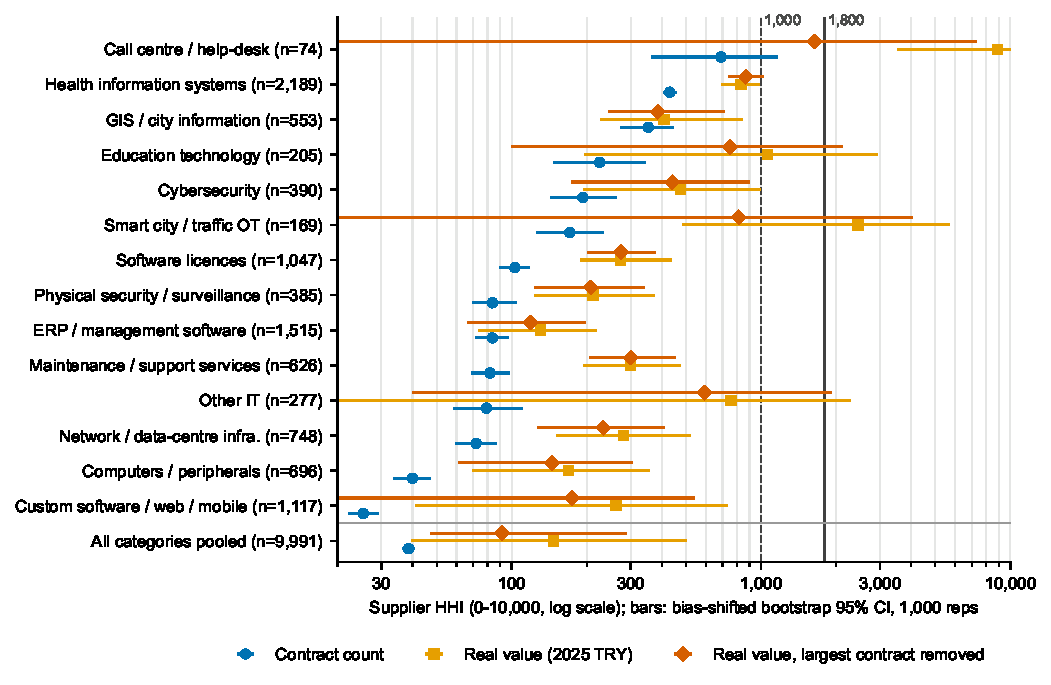
\includegraphics[width=\textwidth]{figures/F-C1_concentration_by_market.pdf}
\caption{Supplier concentration by product market. Points show the HHI by contract count, by real value, and by real value without the market's largest contract; bars are bias-shifted bootstrap 95\% intervals (1,000 resamples). Dashed and solid lines mark 1,000 and 1,800. Log scale.}\label{fig:conc}
\end{figure}

\subsection{Buyers return to incumbents far more often than chance}
Of the 9,991 contracts, 4,913 were awarded by a buyer that had bought in the same product market before. Of these, 45.2\% went to an incumbent supplier. Table~\ref{tab:null} compares this with the null models. Holding each buyer's demand and each firm's wins fixed within product market and year, random assignment would give an incumbency rate of 6.2\% (95\% interval 5.6--6.7\%); the observed rate is 7.3 times higher, which corresponds to about 1,900 contracts won by incumbents beyond the null expectation. Conditioning also on the buyer's sector (N2) raises the null rate to 11.0\%, and conditioning on province (N3), which absorbs local supplier pools, raises it to 20.7\%. Observed incumbency remains 4.1 and 2.2 times higher. The same pattern holds for the share of contracts that fall in repeated pairs (41.5\% observed; 7.1\%, 12.7\%, and 21.6\% under the three nulls) and in every year from 2011 to 2026, where observed incumbency is 5 to 17 times the N1 null (Fig.~\ref{fig:year}).

\begin{table}[t]
\caption{Observed incumbency and repeat contracting against permutation nulls (1,000 permutations each; all $p=0.001$, the minimum attainable).}\label{tab:null}
\begin{tabular}{@{}llrrr@{}}
\toprule
Null model (winners permuted within) & Statistic & Observed & Null mean [95\% interval] & Ratio\\
\midrule
N1: market $\times$ year & Incumbency rate & 0.452 & 0.062 [0.056, 0.067] & 7.3\\
 & Contracts in repeat dyads & 0.415 & 0.071 [0.065, 0.076] & 5.9\\
N2: market $\times$ year $\times$ sector & Incumbency rate & 0.452 & 0.110 [0.103, 0.116] & 4.1\\
 & Contracts in repeat dyads & 0.415 & 0.127 [0.121, 0.133] & 3.3\\
N3: market $\times$ year $\times$ province & Incumbency rate & 0.452 & 0.207 [0.201, 0.213] & 2.2\\
 & Contracts in repeat dyads & 0.415 & 0.216 [0.210, 0.222] & 1.9\\
\botrule
\end{tabular}
\end{table}

Incumbency exceeds its null in every product market (Fig.~\ref{fig:market}). It is highest in health information systems (72\% against a null of 15\%), which alone accounts for 37\% of the excess incumbent contracts, and in maintenance and support services (54\% against 3\%). Enterprise software and software licences follow. By buyer sector, health accounts for 42\% of the excess. The most striking buyers are individual Ministry of Health hospitals and dental centres: in this group 83\% of repeat-eligible contracts go to an incumbent, against a null of 18\%. The results are robust to using recorded rather than split buyer labels (ratio 4.4), original rather than canonicalized firm names (8.4; canonicalization reveals repeats that name variants hide), excluding the call-centre contracts (7.3), adding the ambiguous-scope contracts (7.8), and defining cells by buyer sector instead of product market (9.7).

\begin{figure}[t]
\centering
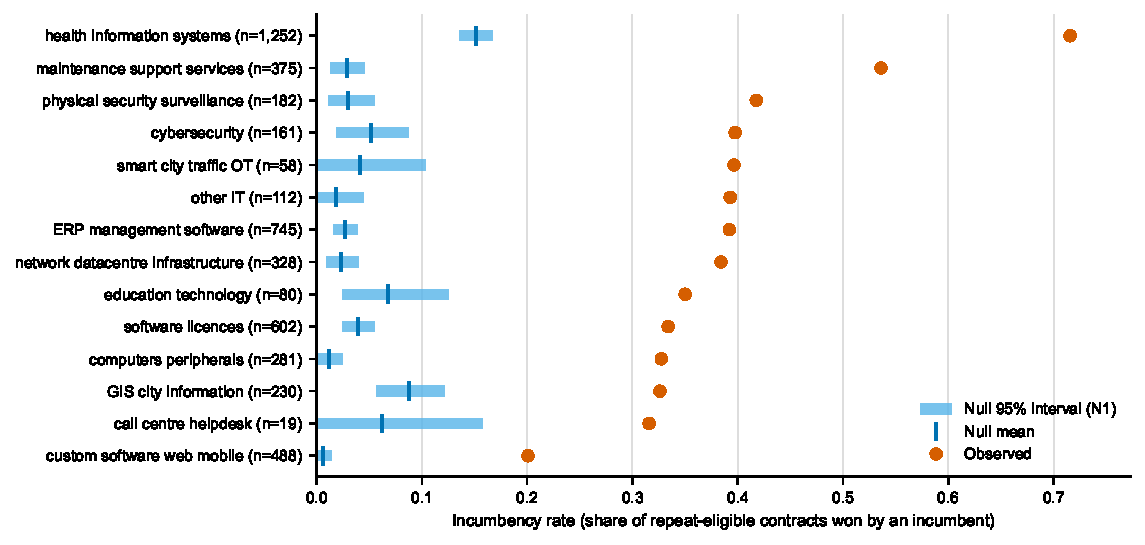
\includegraphics[width=\textwidth]{figures/F_L1_incumbency_by_market.pdf}
\caption{Incumbency rate by product market: observed (dots) and permutation null N1 (mean and 95\% interval; 1,000 permutations within product market $\times$ year). $n$ is the number of repeat-eligible contracts.}\label{fig:market}
\end{figure}

\begin{figure}[t]
\centering
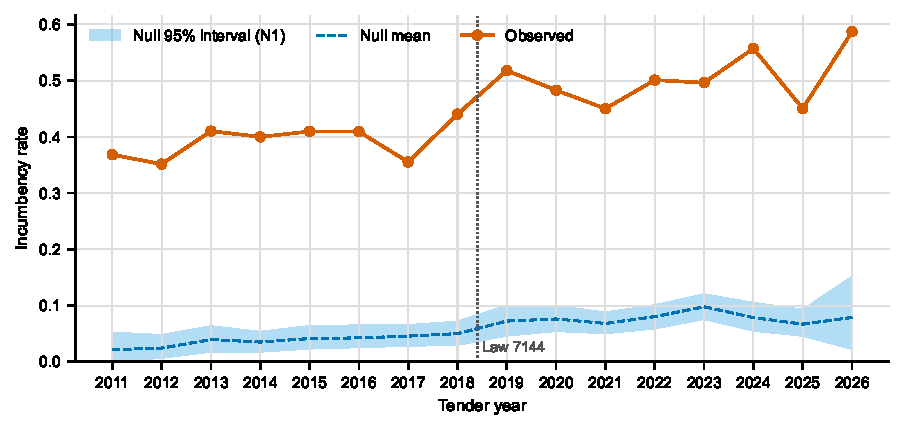
\includegraphics[width=\textwidth]{figures/F_L2_incumbency_by_year.pdf}
\caption{Incumbency rate by year, observed and under null N1 (mean and 95\% interval).}\label{fig:year}
\end{figure}

\subsection{Many buyers depend on one supplier}
The excess is not driven by a few large buyers. Among the 540 buyers with at least five contracts, the median share of the main supplier is 0.33, against a typical null value of 0.16 (Fig.~\ref{fig:buyers}). Fifty-seven percent of these buyers have a main-supplier share above the 95th percentile of their own null distribution, and 70\% have a supplier HHI above it, compared with 5\% expected by chance; under the stricter N2 the shares are 47\% and 61\%. A quarter of these buyers award at least half of their IT contracts to one firm, and 6.5\% award all of them to one firm. Dependence is most pronounced among individual Ministry of Health hospitals and dental centres, where the mean main-supplier share is 0.81 and 90\% of buyers exceed their null. Excess incumbency is present in all size groups of buyers, though somewhat lower for the largest third.

\begin{figure}[t]
\centering
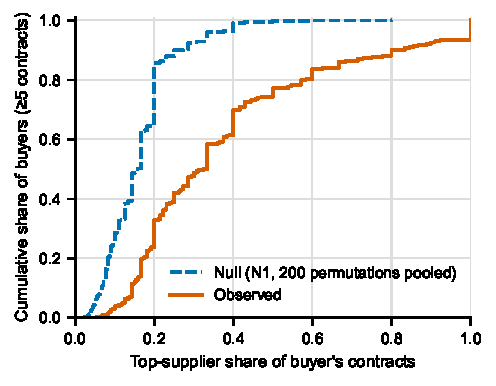
\includegraphics[width=0.8\textwidth]{figures/F_L3_buyer_top_supplier_share.pdf}
\caption{Distribution of the main supplier's share of each buyer's contracts (540 buyers with at least five contracts), observed and under null N1.}\label{fig:buyers}
\end{figure}

\subsection{Procedure, timing, and competition}
Incumbency is higher under Article~21(b) than under open tendering: 72.3\% of repeat-eligible 21(b) contracts go to an incumbent, against 44.1\% of open contracts. The gap of 28 points exceeds its null gap of 9 points ($p=0.001$) and survives the province null. Most excess incumbency nonetheless occurs in open tenders (61\% of excess incumbent contracts, against 19\% under 21(b)), because open tenders are far more numerous. Incumbency is therefore not a feature of the exception route alone.

The difference between procedures is concentrated in time. In the contract-level logit (Table~\ref{tab:logit}), 21(b) contracts were no more likely than open ones to go to an incumbent before 25 May 2018 (average marginal effect $-3.8$ percentage points, 95\% CI $-12.4$ to 4.9), but 13.5 points more likely afterwards (7.2 to 19.9). Raw incumbency under 21(b) rose from 54\% to 81\%. We do not attribute this change to Law No.~7144. A break at the abolition of the hospital unions in August 2017 fits the data slightly better, and a placebo break in 2016 is also significant. Moreover, the interaction is confined to health buyers (odds ratio 2.64 among health buyers, 0.86 among others) and is smaller and imprecise within buyers (7.3 points, $p=0.20$, in a linear probability model with buyer fixed effects). The pattern is consistent with the 2017 reorganization of hospital procurement, after which individual hospitals increasingly renewed IT contracts with their incumbent suppliers through the exception route. It is not consistent with a uniform shift across the public sector.

Incumbency also coincides with weaker competition at the tender stage. In the bid-count sample, 44\% of tenders drew a single bid (95\% CI 39--49\%), 75\% under 21(b) and 41\% under open procedures (Fig.~\ref{fig:single}). Tenders won by an incumbent drew a single bid 71\% of the time (61--80\%), against 32\% (24--42\%) for tenders won by a new supplier; adjusting for procedure and year, the odds ratio is 4.4 (2.4--8.3). The gap is present in open tenders as well (69\% against 37\%). In tenders where the number of firms that obtained the documents is recorded, four firms on average took the documents but fewer than two submitted a valid bid.

\begin{table}[t]
\caption{Logit model of an incumbent win (repeat-eligible contracts). Odds ratios with two-way clustered 95\% confidence intervals (buyer, winning firm).}\label{tab:logit}
\begin{tabular}{@{}lrr@{}}
\toprule
 & Odds ratio [95\% CI] & $p$\\
\midrule
Article 21(b) (vs open) & 0.83 [0.54, 1.28] & 0.401\\
Other negotiated (vs open) & 0.87 [0.70, 1.09] & 0.221\\
Post 25 May 2018 & 1.08 [0.63, 1.85] & 0.773\\
21(b) $\times$ post 25 May 2018 & 2.42 [1.43, 4.09] & $<$0.001\\
Log real value & 0.97 [0.91, 1.05] & 0.451\\
Log prior distinct suppliers of buyer in market & 0.40 [0.30, 0.54] & $<$0.001\\
Log prior contracts of buyer in market & 4.36 [3.47, 5.48] & $<$0.001\\
Years since buyer's first contract in market & 0.89 [0.86, 0.92] & $<$0.001\\
\midrule
Fixed effects & \multicolumn{2}{r}{product market, year, buyer sector}\\
Observations; clusters (buyers, firms) & \multicolumn{2}{r}{4,913; 1,126, 1,437}\\
McFadden pseudo-$R^2$ & \multicolumn{2}{r}{0.17}\\
\botrule
\end{tabular}
\end{table}

\begin{figure}[t]
\centering
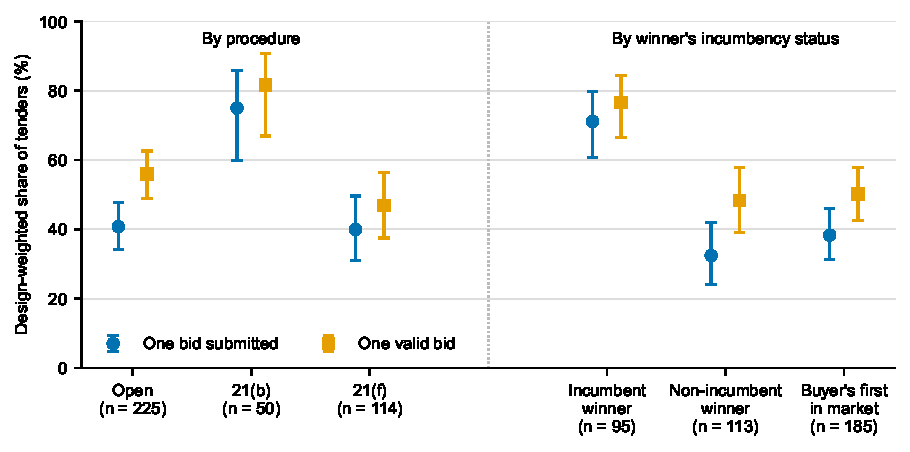
\includegraphics[width=\textwidth]{figures/F-R2_single_bid.pdf}
\caption{Single-bid rates by procedure and by whether the winner was an incumbent (design-weighted, year-stratified sample of 393 tenders, 2012--2026; 95\% intervals).}\label{fig:single}
\end{figure}

\subsection{Network structure}
Figure~\ref{fig:net} shows the core of the buyer--supplier network. The graph is sparse: 5,704 nodes and 7,219 weighted edges, with a giant component that contains 78\% of nodes. Health buyers and health-IT suppliers form a visible cluster, and most other buyers and suppliers are intermixed. Community detection confirms that the network is only moderately modular once its degree structure is taken into account. In the giant component, Louvain modularity is 0.73 on the unweighted graph against 0.69 ($\pm$0.003) in degree-preserving bipartite randomizations; with contract weights the observed value (0.76) is close to the null (0.76). The detected communities align partly with buyer sectors (normalized mutual information 0.25, against 0.03 for permuted labels) and weakly with firms' main product markets (0.13 against 0.04). The structure of the network is therefore mostly what one would expect from a sparse market with many small buyers and specialized suppliers. The relational feature that stands out is not segmentation but the persistence of individual buyer--supplier ties documented above. Brokerage across communities adds little beyond firm size. In several one-mode projections of firms, betweenness is only weakly associated with the number of markets a firm serves once its number of buyers is controlled for (partial Spearman correlations 0.12--0.15), and adding the number of markets to a size-only regression raises $R^2$ by at most 0.015.

\begin{figure}[t]
\centering
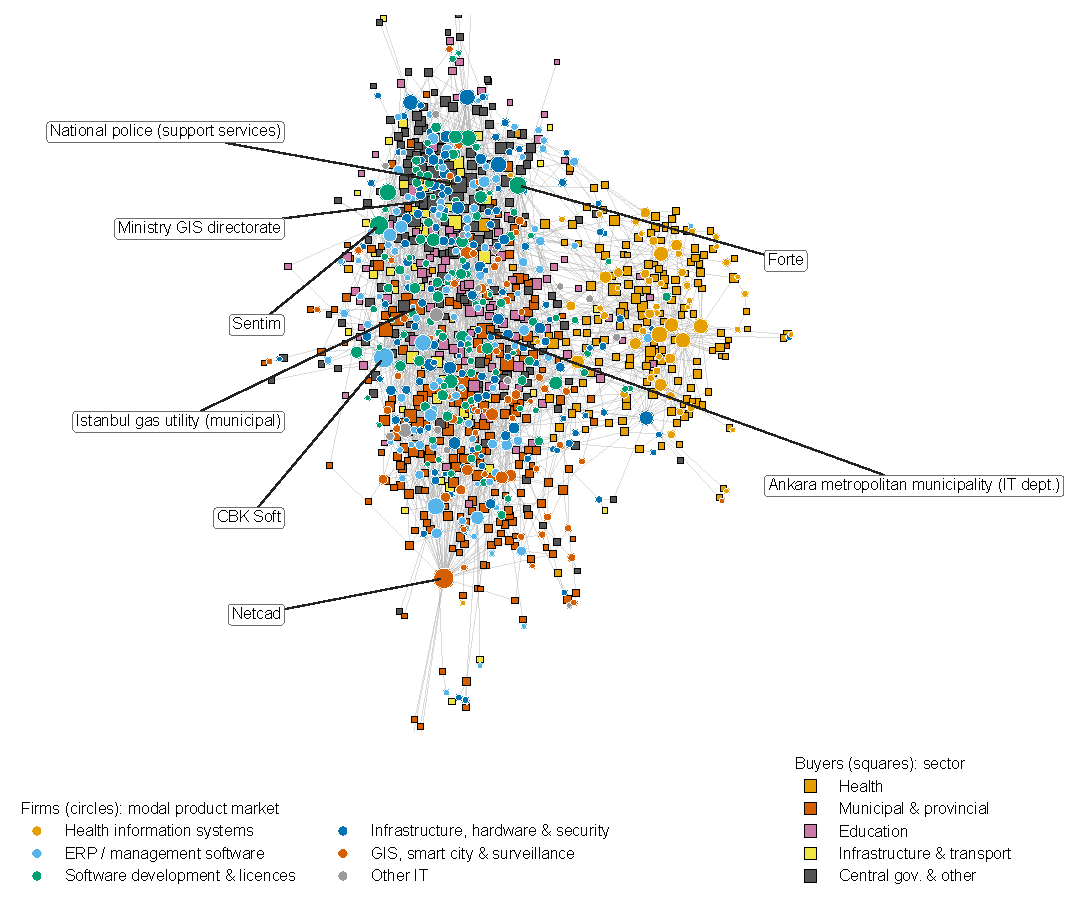
\includegraphics[width=\textwidth]{figures/fig_N1_core_network.pdf}
\caption{Core of the buyer--supplier network (giant component, nodes of degree $\geq 3$; force-directed layout with fixed seed). Circles are firms coloured by their main product market; squares are buyers coloured by sector; size reflects degree.}\label{fig:net}
\end{figure}

\section{Discussion}\label{sec:discussion}

\subsection{Interpretation}
The central result is a divergence between two levels of analysis. At the level of markets, Turkish public IT procurement is not concentrated: hundreds of firms compete, no product market passes the conventional thresholds on robust measures, and pooled indices are very low. At the level of buyers, the same market shows persistent relationships. Buyers return to their previous suppliers at several times the rate that market structure, timing, sector, and even local supplier pools would produce. The two findings are not contradictory. Market shares measure how supply is distributed across all buyers; incumbency measures how narrow the choice of each buyer is. A market in which each buyer is tied to a different supplier can have low concentration and high dependence at the same time.

Several mechanisms can produce excess incumbency, and our data do not separate them fully. The most benign is legitimate continuity. Maintenance, licence renewals, and extensions of installed systems are often best provided by the original supplier, and the concentration of excess incumbency in hospital information systems and in maintenance services fits this switching-cost account \citep{Greenstein1993,FarrellKlemperer2007}. A second mechanism is information: buyers may prefer suppliers whose performance they know, which can improve outcomes \citep{Coviello2018}. A third is the erosion of competition. Incumbent-won tenders are much more likely to attract a single bid, and many firms that obtain tender documents do not bid. Our data record winners and bid counts but not the identities of losing bidders, so we cannot tell whether other firms were deterred, excluded, or simply uninterested. The single-bid gap is consistent with incumbency advantages that discourage entry, but it is also what one would expect if only the incumbent can supply a proprietary system.

The role of Article~21(b) illustrates the limits of procedure as an explanation. The exception route has the highest incumbency rate, and its link with incumbency strengthened after 2017. Yet most excess incumbency arises in open tenders, the post-2017 change is specific to health buyers, and within buyers the association is weak. Discretionary procedures thus appear to be one channel through which existing relationships are renewed, rather than the source of the relationships themselves.

\subsection{Implications for monitoring}
Procurement monitoring in Türkiye, as elsewhere, relies on market-level statistics and on procedural red flags such as single bidding \citep{fazekas2016objective,FazekasKocsis2020}. Our results suggest adding a buyer-level layer. Buyer-level incumbency rates and dependence on the main supplier can be computed from the same award records, and they can be benchmarked against permutation nulls like ours to separate genuine persistence from what market size and specialization imply. Such indicators would direct attention to specific buyers and product markets, above all hospital information systems, where exit options are limited. The appropriate response is not necessarily more tendering. Where switching costs are real, policies that lower them may do more for competition than additional procedures. Examples are data-portability and interoperability requirements for health information systems, and contract terms that separate system licences from maintenance.

\subsection{Limitations}
Our analysis is descriptive and associational. Incumbency is measured from winners only: without the identities of losing bidders we cannot model bidding behaviour or detect collusion, and the bid-count sample is small and starts in 2012. Scope is defined by keywords and a value-based audit, and about 1,400 ambiguous contracts were excluded from the main sample; including them does not change the results. Firm names were canonicalized by rules and a manual review of the largest firms, without tax identifiers, so some duplicates may remain; canonicalization increases rather than decreases measured incumbency. Buyers are identified by their recorded names, and splitting pooled labels by province is an approximation. The product-market classification is based on tender titles. Values are deflated with the general consumer price index. Finally, the timing results cannot distinguish between Law No.~7144, the 2017 health reorganization, and a secular trend.

\section{Conclusion}\label{sec:conclusion}
Türkiye's public IT market is unconcentrated by conventional measures, yet its buyers are frequently captive to their incumbent suppliers. Among contracts that could go to a returning supplier, 45\% do, several times the rate that market structure implies. The excess is largest in health IT and in negotiated procurement without publication, and incumbent-won tenders rarely attract competing bids. Market-level concentration indices are therefore an incomplete guide to competition in public procurement. Buyer-level incumbency, measured against an appropriate null, identifies where dependence arises and where policies that lower switching costs could matter most.

\backmatter

\bmhead{Supplementary information}
The Supplementary Information contains the scope audit, entity resolution, product-market classification, full concentration tables, all null-model results and sensitivities, the dyad-continuation model and specification tests, the single-bid sample design, and additional network analyses.

\bmhead{Acknowledgements}
This study grew out of a term project in the SE~434 Social Network Analysis course at Maltepe University. We thank Assist.\ Prof.\ Dr.\ Volkan Tunal\i{} for his guidance during the course and for comments on early versions of the analysis.

\section*{Declarations}

\begin{itemize}
\item \textbf{Funding.} This research received no specific grant from any funding agency in the public, commercial, or not-for-profit sectors.
\item \textbf{Competing interests.} The authors have no competing interests to declare.
\item \textbf{Ethics approval.} Not applicable. The study uses public administrative records. Names of natural persons are pseudonymized in the released data.
\item \textbf{Data and code availability.} Code, derived data, and a data dictionary are available at \url{https://github.com/XXXX/TenderNet} and archived on Zenodo (\url{https://doi.org/10.5281/zenodo.XXXXXXX}). The underlying records are published by the Public Procurement Authority on EKAP (\url{https://ekapv2.kik.gov.tr}).
\item \textbf{Use of AI tools.} Claude (Anthropic) was used to assist with analysis code, figure preparation, and language editing. The authors designed the study, checked all code and results, and take full responsibility for the content.
\item \textbf{Author contributions.} F.A.: conceptualization, methodology, data curation, software, formal analysis, visualization, writing (original draft, review and editing). A.Ş.: data curation, investigation, validation, visualization, writing (review and editing).
\end{itemize}

\bibliography{refs}

\end{document}
